\begin{figure}[h]
    \centering
    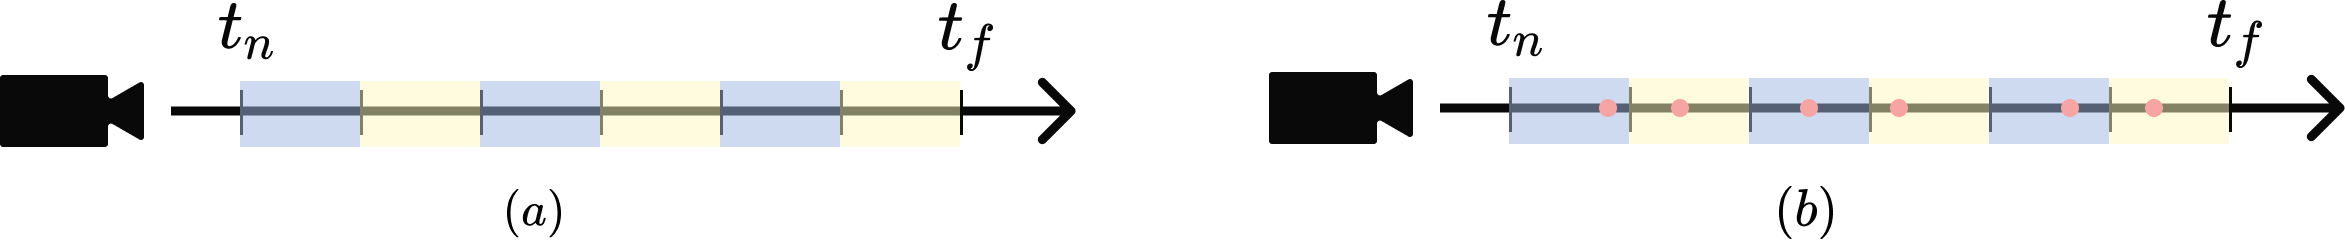
\includegraphics[width=1.0\textwidth]{figures/stratified-sampling.png}
    \caption[Stratified sampling]{Illustration of stratified sampling. a) The ray is uniformly binned from the near bound $t_n$ to the far bound $t_f$ of a ray $r(t)$, defining the strata. b) A single random point is randomly sampled from each stratum.}
    \label{fig:stratified-sampling}
\end{figure}